\documentclass[uplatex, dvipdfmx, a4paper, report, papersize, 11pt]{jsbook}
\usepackage{bm}
\usepackage{amsmath}
\usepackage[dvipdfmx]{graphicx}
\usepackage{wrapfig}
\usepackage[hang, small, bf]{caption}
\usepackage[subrefformat=parens]{subcaption}
\usepackage{here}
\usepackage{comment}
\captionsetup{compatibility=false}

\bibliographystyle{jplain}
\title{二色の光周波数コムによるレーザー冷却法の開拓}
\author{物理工学科4年 中西亮}
\date{2019/1/30}
\begin{document}
\maketitle
\newpage

\setcounter{tocdepth}{2}
\tableofcontents


\newpage
\chapter{過去の研究に基づくCs原子の二光子冷却のシミュレーション}
\section{従来の課題と光周波数コムによる冷却のメリット}

 従来のレーザー冷却では, アルカリ金属やアルカリ土類金属などの限られた原子しか冷却できなかった.この理由としては主に2つの理由が挙げられる. 1つ目としては, 水素や酸素を含む多くの原子の遷移エネルギーは真空紫外領域に相当しており現在はこの領域で十分な強度のレーザーを得ることができていないことがある. 2つ目は, 多くの原子ではエネルギー準位の構造が複雑であり励起された原子が準安定な準位に緩和してしまうので, これを励起するためのレーザーを用意する必要があり実験の系が複雑化してしまうことである\cite{PhysRevA.73.063407}.\\
 光周波数コムを用いた二光子のレーザー冷却は, 2006年にKielpinski\cite{PhysRevA.73.063407}によって提案された. 光周波数コムを用いることにより, 上記の2つの課題を克服することができる. まず, 光周波数コムは高強度のピークパワーをもつため, 同じ時間平均パワーをもつcwレーザーに比べて高効率の非線形工学効果を利用することができ, より高強度の短波長のレーザーを得ることができる. また, 光周波数コムの一つ一つのの縦モードがリポンプレーザーとして機能するために, 実験の系を簡単にすることができる. これらの長所により, 光周波数コムはcwレーザーよりも効率の良い二光子冷却を実現することができる\cite{PhysRevA.73.063407}.\\
 本章では, コムを用いた二光子冷却についての過去の研究の内容を紹介する.

\section{二光子コムによるレーザー冷却の理論}
 Jayichらの論文\cite{PhysRevX.6.041004}で説明されている, 二光子遷移を用いたレーザー冷却の理論を紹介する.\\
コムによる二光子の遷移を考えるとき, パルスに含まれる二光子のエネルギーもまた, コム(櫛)を形成する.これを二光子コムと呼ぶことにすると, 二光子コムのn番目の縦モードの周波数は
\begin{equation}
f_n = nf_r + 2f_0
\end{equation}
となる. ただし, $f_r$:は繰り返し周波数, $f_0$はキャリアエンベロープオフセット周波数を表す.チャープのモード同期レーザーについては実効的な共鳴ラビ周波数を求めることができる. 二光子コムのn番目のコムの歯共鳴ラビ周波数は,
\begin{eqnarray}\label{ResonanceRabi}
\Omega _{n} &=&\sum _{p}\frac {g^{\left( 1\right) }_{p}g^{\left( 2\right) }_{n-p}}{2\Delta_p} \nonumber\\
&=& \sum _ { p } \frac { e ^ { 2 } \mathcal { E } _ { p } \mathcal { E } _ { n - p } } { \hbar ^ { 2 } } \left\langle \mathrm { e } \left| ( \hat { \boldsymbol { \epsilon } } \cdot \mathbf { r } ) \left( \sum _ { \mathrm { i } } \frac { | \mathrm { i } \rangle \langle \mathrm { i } | } { 2 \Delta _ { p } ^ { ( \mathrm { i } ) } } \right) ( \hat { \boldsymbol { \epsilon } } \cdot \mathbf { r } ) \right| \mathrm { g } \right\rangle
\end{eqnarray}\\
ただし, $g^{\left( 1\right) }_{p}$は$p$番目のコムの歯による基底状態から中間状態への共鳴一光子ラビ周波数, $g^{\left( 2\right) }_{p}$は$p$番目のコムの歯による中間状態から励起状態への共鳴一光子ラビ周波数を表す.
$\Delta _{p}=pf_{r}+f_{0}-f_{gi}$は一光子の中間状態からの離調である. ただし, $f_{gi}$は基底状態から中間状態へのエネルギー差をプランク定数$h$で割ったものである.また、$\epsilon_0$は真空の誘電率、$c$は光速、$e$は電気素量、$\hbar$はプランク定数$h$を$2\pi$で割った値を表す。\\
二光子コムのN番目のコムの歯が共鳴周波数に最も近いとき, 速度$v$で動く原子の励起確率の時間平均は,
\begin{equation}\label{ExcitationRate}
\gamma_\mathrm{comb} = \frac{\Omega^2_{N}T_\mathrm{r}} {4} \frac{\sinh(\gamma T_\mathrm{r}/2)}{\cosh(\gamma T_\mathrm{r}/2) - \cos(\delta_N(\bm{v})T_\mathrm{r})}
\end{equation}
ここで, $\delta _{N}\left( v\right) \equiv 2\pi ( f_\mathrm{\mu }-f_\mathrm{ge}-f_{N}\widehat {\bm{k}}\cdot {\bm{v}}/c )$は$N$番目の二光子コムの歯の共鳴周波数からの離調を表す.$f_{ge}$は励起状態と基底状態のエネルギー差をプランク定数で割ったもの, $\widehat {\bm{k}}$はレーザーの進行方向の単位ベクトル, $\gamma$は励起準位の自然幅を表す.\\
離調$\delta _{N}\left( v\right)$と自然幅$\gamma$の両方がコムの歯の間隔($2\pi f_r$)よりも小さいとき, 二光子コムは二光子ラビ周波数$\Omega_N$の一つの縦モードとして扱うことができる.この近似の下では, 励起確率は
\begin{equation}\label{EffectiveExcitationRate}
\gamma_N = \frac{\Omega^2_N}{\gamma}\frac{1}{1 + [2\delta_N(\bm{v})/\gamma]^2}
\end{equation}
と表せる.\\
 また, (二色のコムによる冷却ではなく)縮退したコムによる二光子冷却の場合, ドップラー冷却限界温度は
\begin{equation}
  T_\mathrm{D} = \frac{3}{4}\frac{\hbar\gamma}{2k_\mathrm{B}}
\end{equation}
となることが分かっている. ただし, $k_\mathrm{B}$はボルツマン定数\\
 Jayichらの論文\cite{PhysRevX.6.041004}では, 初めて光周波数コムを用いた二光子冷却の実証実験が行われた.Jayichらのグループはルビジウムの縮退した二光子のコムによる一次元のレーザー冷却に成功し, 57 $\mu$Kを達成している.

\section{Cs原子の冷却に必要な励起効率の見積もり}
  今回はあらかじめMOTで予冷されたCs原子を冷却することを目指すが、その際に必要な二光子遷移の励起効率を見積もる。$6 ^ { 2 } S _ { 1 / 2 }$の$F = 4$から$6 ^ { 2 } P _ { 3 / 2 }$の$F ^ { \prime } = 5$の遷移によるドップラー冷却を行った場合、ドップラー冷却温度は$125.61\ \mathrm{\mu K}$となる\cite{Cs_level_diagram}。このことから、二光子コム照射時のCs原子の温度は数百$\mathrm{\mu K}$以下にできると考えられる。原子の温度が$T$ Kのときの原子の速さの最頻値は
\begin{equation}
  v _ { \mathrm { th } } = \sqrt { \frac { 2 k _ { \mathrm { B } } T } { m }}
\end{equation}
で与えられる。ただし、mは原子の質量を表す。MOT後の原子の速さはこの最頻値を持つものとして計算する。例えば、$126\ \mathrm{\mu K}$のCs原子の速さの最頻値は$125$ mm/sである。また6s軌道から8s軌道への二光子遷移を利用して冷却する場合、二つの光子の周波数が同じであるとすると822nm程度の波長を持つ。この場合二光子を吸収した時のCs原子の速度変化は二光子を吸収するごとに$7.3$ mm/s程度の減速である。
ドップラー冷却における加熱効果を無視して、近似的に原子が等加速度$a\ \mathrm{m/s^2}$で減速するとすると、速度$v$を持つ原子が停止するまでに移動する距離$l$は
\begin{equation}
    l = \frac{v^2}{2a}
\end{equation}
で与えられる。実験で用いるレーザーの直径を考慮して原子が冷却されるまでに$0.5$ mm以内の移動距離に抑えるのに必要な加速度から冷却に必要な励起効率を初期温度に応じて計算すると、図\ref{necessary_excitation_rate}のようになる。この結果と実験上のロスを考慮して今回の実験では$10000\ \mathrm{s^{-1}}$の励起効率を目標とする。
\begin{figure}[htpb]
  \centering
    \begin{tabular}{c}
      \begin{minipage}{1\hsize}
        \centering
          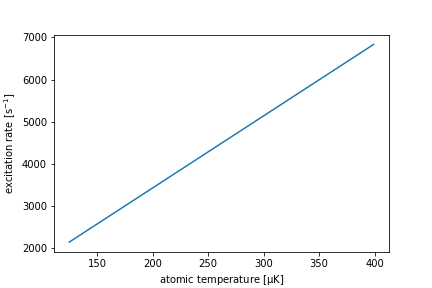
\includegraphics[keepaspectratio,  scale=0.6,  angle=0]
                          {figures/chapter3/necessary_excitation_rate.png}
                          \caption{MOTで予冷したCs原子の冷却に必要な励起効率。計算の詳細については本文中に記載。}
                          \label{necessary_excitation_rate}

      \end{minipage}
    \end{tabular}
\end{figure}
\section{Cs原子の二色のコムによる励起効率の見積もり}
 Jayichらの論文\cite{PhysRevX.6.041004}では、Rb原子の5s軌道から5d軌道への遷移を利用しており、以下のパラメータの下で実験を行っている。
\begin{itemize}
  \item 5d順位の線幅 : $2\pi \times 667$ kHz
  \item コムのパルス幅 : $2-5$ ps
  \item コムの平均パワー : $500$ mW
  \item コムビームの直径 : $1$ mm
  \item コムの周波数帯域 : $500$ GHz
  \item コムの繰り返し周波数 : $80$ MHz
\end{itemize}
Jayichらはこのパラメータの下で励起効率を$\gamma_N \sim 13000\ \mathrm{s^{-1}}$と見積もっている。\\
 Jayichらの論文\cite{PhysRevX.6.041004}の励起確率の計算手法に習い、今回私達の用いるコムでCs原子を冷却する際の励起確率の計算を行った。その計算に際して以下の五つの近似を行った。\\
\\
 (a) $\delta_N(\bm{v}) = 0$とし、
\begin{equation}
  \gamma_N = \frac{\Omega^2_N}{\gamma}
\end{equation}
     とした。\\
 (b) 二光子励起の際の中間状態として$6P_{\frac{3}{2}}$以外の状態を無視した。\\
 (c) 光周波数コムの全ての縦モードの電場の強さが一定であるとして計算を行った。
\begin{equation}
  \mathcal{E}_p = const.
\end{equation}
 (d) 以下の関係式を用いた。
\begin{equation}
  \Sigma_{p} \mathcal{E}_p\mathcal{E}_{n-p} \approx 2I/\epsilon_0 c
\end{equation}
 (e) $\left\langle \mathrm { e } \left| ( \hat { \boldsymbol { \epsilon } } \cdot \mathbf { r } ) | \mathrm { i } \rangle \langle \mathrm { i } |  ( \hat { \boldsymbol { \epsilon } } \cdot \mathbf { r } ) \right| \mathrm { g } \right\rangle$ の値がCs原子とRb原子で等しいとした。\\
\\
 (a)-(d)の近似を用いると、励起効率の式(\ref{EffectiveExcitationRate})は以下のように計算できる。\\
\begin{eqnarray}\label{approx_ex-rate}
  \gamma_N &=& \frac{\Omega^2_N}{\gamma}\frac{1}{1 + [2\delta_N(\bm{v})/\gamma]^2} \nonumber\\
  &=& \frac{\Omega^2_N}{\gamma}  \nonumber\\
  &=& \frac{1}{\gamma} \Biggl[ \sum _ { p } \frac { e ^ { 2 } \mathcal { E } ^{(1)}_ { p } \mathcal { E }^{(2)} _ { N - p } } { \hbar ^ { 2 } } \left\langle \mathrm { e } \left| ( \hat { \boldsymbol { \epsilon } } \cdot \mathbf { r } ) \left(  \frac { | \mathrm { i } \rangle \langle \mathrm { i } | } { 2 \Delta _ { p } ^ { ( \mathrm { i } ) } } \right) ( \hat { \boldsymbol { \epsilon } } \cdot \mathbf { r } ) \right| \mathrm { g } \right\rangle \Biggr]^2 \nonumber \\
  &=& \frac{1}{\gamma} \Biggl[ \sum _ { p } \frac { e ^ { 2 } \mathcal { E }^{(1)} \mathcal { E } ^ {(2)} } { \hbar ^ { 2 } } \left\langle \mathrm { e } \left| ( \hat { \boldsymbol { \epsilon } } \cdot \mathbf { r } ) \left(  \frac { | \mathrm { i } \rangle \langle \mathrm { i } | } { 2 \Delta _ { p } ^ { ( \mathrm { i } ) } } \right) ( \hat { \boldsymbol { \epsilon } } \cdot \mathbf { r } ) \right| \mathrm { g } \right\rangle \Biggr]^2 \nonumber \\
  &=& \frac{e^2  \mathcal { E } ^ {(1)} \mathcal { E } ^ {(2)}}{ 2 \gamma \hbar ^ { 2 }  }\Biggl[ \left\langle \mathrm { e } \left| ( \hat { \boldsymbol { \epsilon } } \cdot \mathbf { r } ) | \mathrm { i } \rangle \langle \mathrm { i } |  ( \hat { \boldsymbol { \epsilon } } \cdot \mathbf { r } ) \right| \mathrm { g } \right\rangle\sum _ { p }\frac{1}{2 \Delta _ { p } ^ { ( \mathrm { i } ) }} \Biggr]^2\\
  \mathcal{E}^{(i)} &=&  \sqrt{\frac{2 I_{i}}{M \epsilon_0 c}}\ \ \ \ (i = 1,2)
\end{eqnarray}\\
ただし、$\mathcal{E}^{(1)}_p$は基底状態から中間状態へのコムの$p$番目の縦モードの電場の大きさを表し、、$\mathcal{E}^{(2)}_p$は中間状態から励起状態へのコムの$p$番目の縦モードの電場の大きさを表す。$\mathcal{E}^{(i)}\ \ (i = 1,2)$は近似(c)の下でのコムの電場の強さを表す。$I_{i}\ \ (i = 1,2)$はそれぞれのコムの強度を表す。$M$はコムの歯の本数を表し、計算上では2つのコムの歯の数は等しいとした。\\
 まず、Jayichらのグループが計算で得た励起効率から計算すると
\begin{equation}
\left\langle \mathrm { e } \left| ( \hat { \boldsymbol { \epsilon } } \cdot \mathbf { r } ) | \mathrm { i } \rangle \langle \mathrm { i } |  ( \hat { \boldsymbol { \epsilon } } \cdot \mathbf { r } ) \right| \mathrm { g } \right\rangle = 4.1 \times 10^{-22} \mathrm{m^2}
\end{equation}
を得る。この値をCsでも用いて計算する。\\
 今回の実験ではCsの$6S_{1/2}$から$8S_{1/2}$の二光子遷移を利用して冷却を行う。まず、中心波長$822$ nmの同じコムから二光子を吸収した場合での励起効率の計算を行った。このときのパラメータを以下に示す。
\begin{itemize}
  \item 遷移 : $6S_{1/2}$から$8S_{1/2}$
  \item 8S順位の線幅 : $2\pi \times 2.18$ MHz
  \item コムビームの直径 : $1$ mm
  \item コムの周波数帯域 : $20$ THz
  \item コムの繰り返し周波数 : $120$ MHz
  \item 中間状態の$6P_{\frac{3}{2}}$への遷移周波数は852nmとする。
\end{itemize}
以上の条件の下で、式(\ref{approx_ex-rate})を用いて二光子励起効率のコムのパワー依存性を計算すると図\ref{degenerated_2_photon_excitation_rate-P}のようになる。このグラフから、励起効率が不足していることが分かる。\\
\begin{figure}[htpb]
  \centering
    \begin{tabular}{c}
      \begin{minipage}{1\hsize}
        \centering
          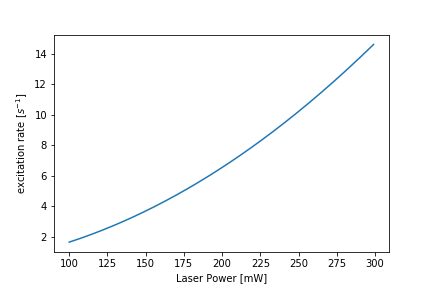
\includegraphics[keepaspectratio,  scale=0.6,  angle=0]
                          {figures/chapter3/degenerated_2_photon_excitation_rate-P.png}
                          \caption{縮退した二光子で冷却した場合の励起効率。計算の詳細は本文中に記載。}
                          \label{degenerated_2_photon_excitation_rate-P}
      \end{minipage}
    \end{tabular}
\end{figure}


\section{二色のコムによる励起に必要なパワーの見積もり}
\subsection{一光子遷移による中間状態への励起効率の見積もり}
 上述のシミュレーションで励起効率が低下した要因としては、中間状態である$6P_{\frac{3}{2}}$からの一光子コムの離調が大きいことが挙げられる。このことから、周波数の異なる二つの光子による励起により中間状態からの一光子コムの離調を小さくすることで励起効率を向上させることができるのではないかと考えられる。しかし、二色のコムで冷却する場合は一光子コムの歯と中間状態の離調をどの程度まで小さくできるかについても注意する必要がある。なぜなら、あまりに離調を小さくしすぎると中間状態に電子が励起される一光子励起の過程が支配的になってしまうからである。離調をどの程度まで小さくできるかについては一光子の散乱効率を評価することで判断した。二光子冷却時のレーザーの照射時間は、Jayichらの論文での冷却時間を参考にして5msであると仮定する。このレーザーの照射時間における一光子の散乱回数が$1$以下になることを期待すると、散乱効率は$200\ \mathrm{s^{-1}}$以下である必要がある。\\
 散乱効率は次の式で与えられる。
\begin{equation}
  R _ { \text { scatt } } = \frac { \Gamma } { 2 } \frac { \Omega ^ { 2 } / 2 } { \delta ^ { 2 } + \Omega ^ { 2 } / 2 + \Gamma ^ { 2 } / 4 }
\end{equation}
この式は飽和パラメーター$s$を用いて
\begin{equation}
  R _ { \text { scatt } } = \frac { \Gamma } { 2 } \frac{s}{1+s}
\end{equation}
と表せる。$s$は吸収遷移の飽和強度$I_0$と用いるレーザーの強度$I$により、
\begin{equation}
  s = \frac{I/I_0}{1+(2\delta/\Gamma)^2}
\end{equation}
と書けるのでこれを用いて計算する\cite{ノーベル賞と分光学}。なお、予めMOTで冷却済みのためドップラー効果の寄与は無視した。Cs原子の中間状態は$6P_{\frac{1}{2}}$($\Gamma = 4.56$ MHz,\ $I_0 = 2.50 \mathrm{\ mW/cm^2}$)を用いた\cite{CsDLine}。また、強度については近似 (c)を用いて、全体の強度をコムの歯の数で割ったものを一本のコムの歯の強度として、全てのコムの歯における$R _ { \text { scatt } }$を独立に計算し、その総和をコム全体の$R _ { \text { scatt } }$とした。この際の、コムの周波数幅は$6S_{\frac{1}{2}}$から$6P_{\frac{1}{2}}$
の共鳴周波数付近で$10$ nm程度の波長幅に対応する$5$ THzとした。繰り返し周波数$f_{\mathrm{rep}}$については当実験室にある二種類のコムの繰り返し周波数である$120$ MHzと$1.6$ GHzにおいて計算を行った。その結果を示したのが図\ref{1photon-sc-rate-2dcolor_120MHz_log},\ref{1photon-sc-rate-2dcolor_16GHz_log}である。\\
\begin{figure}[H]
  \centering
    \begin{tabular}{c}
      \begin{minipage}{1\hsize}
        \centering
          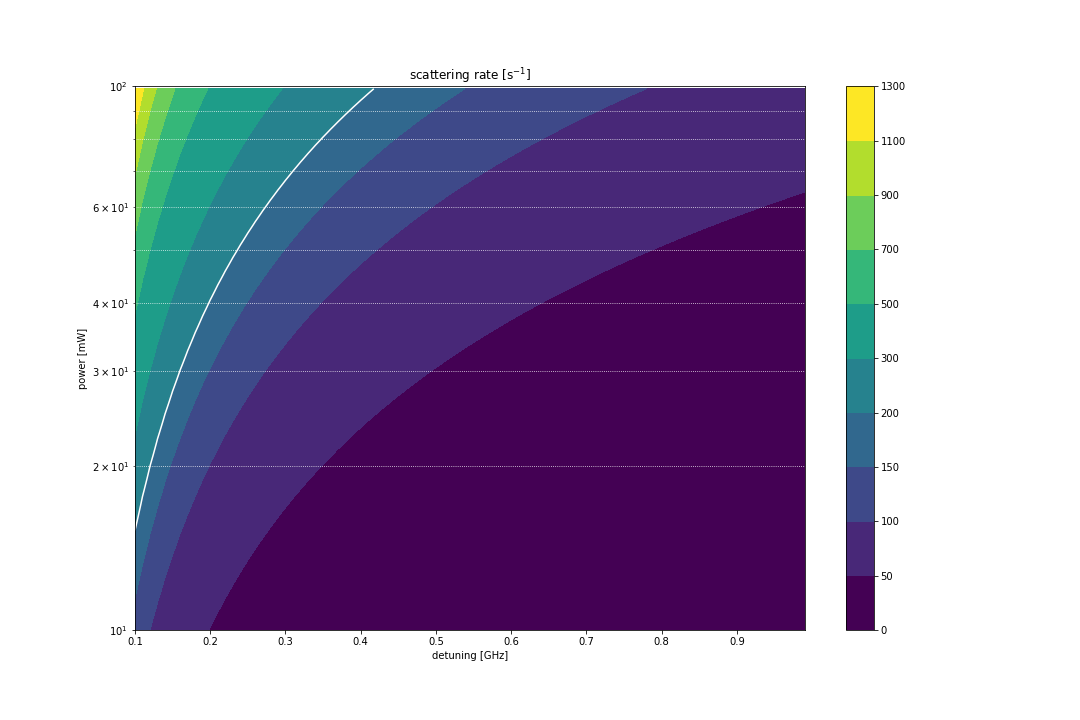
\includegraphics[keepaspectratio,  scale=0.35,  angle=0]
                          {figures/chapter3/1photon-sc-rate-2dcolor_120MHz_log.png}
                          \caption{中間状態への励起効率の離調とパワー依存性。横軸は$6S_{\frac{1}{2}}$から$6P_{\frac{1}{2}}$の共鳴にもっとも近い一光子コムの歯と$6P_{\frac{1}{2}}$の離調を示している。コムの周波数幅は$5$ THz, $f_{\mathrm{rep}}$は$120$ MHzとしている。グラフ中の白い実線が励起効率$200\ \mathrm{s^{-1}}$を表す。}
                          \label{1photon-sc-rate-2dcolor_120MHz_log}
      \end{minipage}\\
      \begin{minipage}{1\hsize}
        \centering
          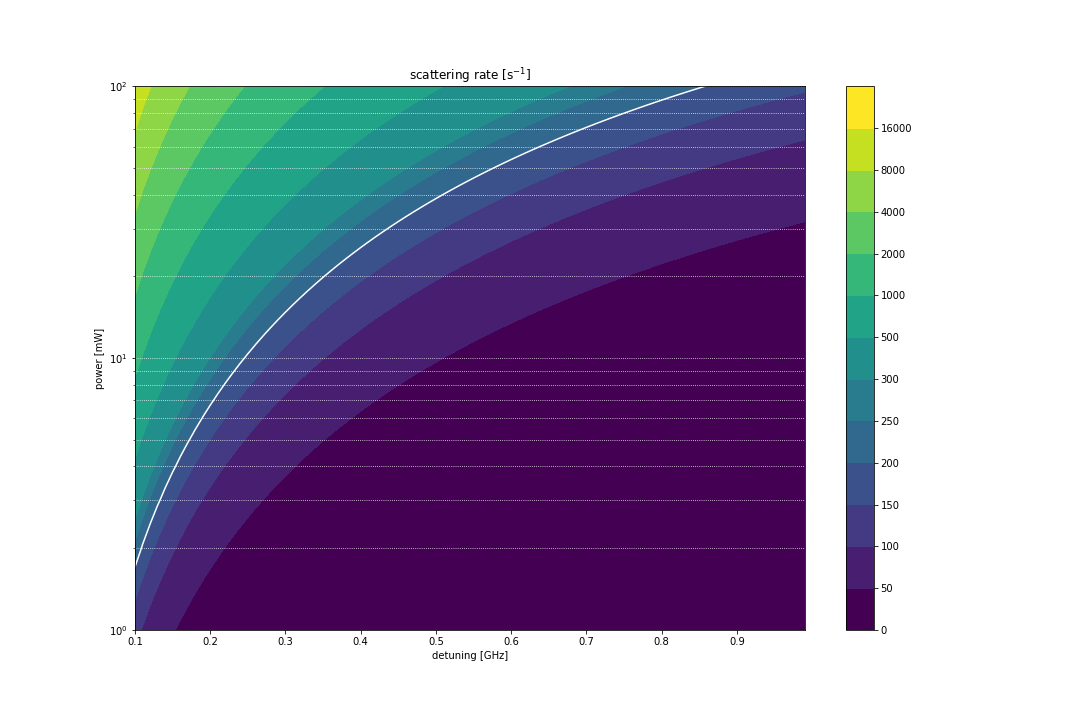
\includegraphics[keepaspectratio,  scale=0.35,  angle=0]
                          {figures/chapter3/1photon-sc-rate-2dcolor_16GHz_log.png}
                          \caption{中間状態への励起効率の離調とパワーの依存性。横軸は$6S_{\frac{1}{2}}$から$6P_{\frac{1}{2}}$の共鳴にもっとも近い一光子コムの歯と$6P_{\frac{1}{2}}$の離調を示している。コムの周波数幅は$5$ THz, $f_{\mathrm{rep}}$は$1.6$ GHzとしている。グラフ中の白い実線が励起効率$200\
                          \mathrm{s^{-1}}$を表す。}
                          \label{1photon-sc-rate-2dcolor_16GHz_log}
      \end{minipage}
    \end{tabular}
\end{figure}
\newpage
\subsection{二色のコムによる冷却に必要なパワーの見積もり}
このように波長の異なるコムを用意するには、周波数幅の広いコムからバンドパスフィルター(BPF)を用いて目的の周波数帯を取り出す必要がある。しかし、単に切り出すだけでは光のパワーが低下してしまい励起効率が低下することが予想される。そのため、二色のコムを用いて励起する場合二色のどのような強度のコムを用意すると目標の励起効率が得られるのかのシミュレーションを行った。その際前節の議論を踏まえ、$f_{\mathrm{rep}} = 120$ MHzのコムでは、$6P_{\frac{1}{2}}$と最近接の一光子コムの歯の離調が$200$ MHz, $400$ MHzの際の励起効率を二つのコムのパワーに応じて計算した。この際、一光子の$6P_{\frac{1}{2}}$への散乱効率が$1 \mathrm{s^{-1}}$よりも大きくならないように注意して、$894$ nm側のコムのパワーを設定した。計算の結果を図\ref{5THz-120MHz-04GHz_new}, \ref{5THz-120MHz-02GHz_new}, \ref{5THz-16GHz-04GHz_new}, \ref{5THz-16GHz-08GHz_new}に示す。この計算結果から$10000 \mathrm{s^{-1}}$の励起効率を得るために、必要な二色のコムのパワーと中間状態からの一光子コムの歯の離調のおよその組み合わせを見積もることができた。\\
\newpage
\begin{figure}[H]
  \centering
    \begin{tabular}{c}
      \begin{minipage}{1\hsize}
        \centering
          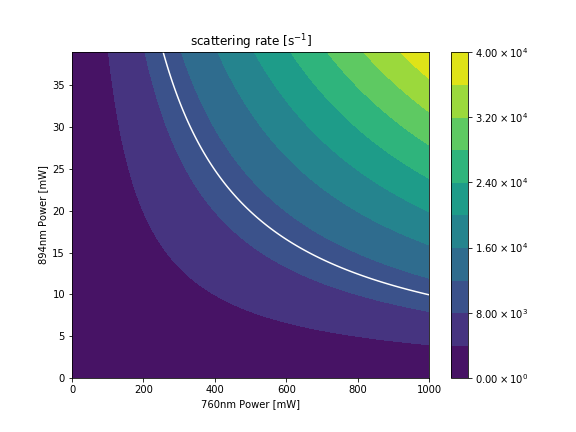
\includegraphics[keepaspectratio,  scale=0.6,  angle=0]
                          {figures/chapter3/2dcolor/5THz-120MHz-02GHz_new.png}
                          \caption{$f_\mathrm{rep} = 120\ \mathrm{MHz}$で$6P_{\frac{1}{2}}$と最近接の一光子コムの歯の離調が$200$ MHzのときの、二光子励起効率のパワー依存性。図中の白い実線が$10000\ \mathrm{s^{-1}}$の励起効率を示す。}
                          \label{5THz-120MHz-02GHz_new}
      \end{minipage}\\
      \begin{minipage}{1\hsize}
          \centering
            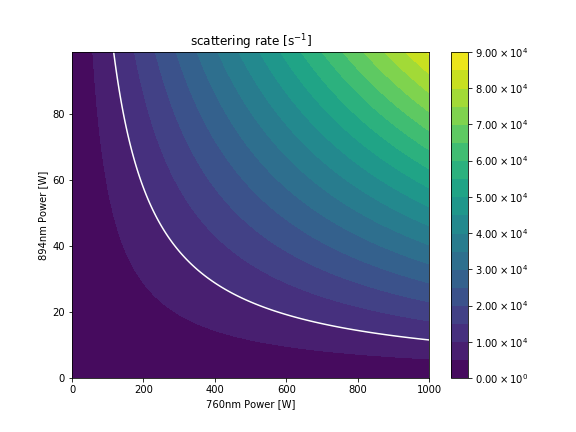
\includegraphics[keepaspectratio,  scale=0.6,  angle=0]
                            {figures/chapter3/2dcolor/5THz-120MHz-04GHz_new.png}
                            \caption{$f_\mathrm{rep} = 120\ \mathrm{MHz}$で$6P_{\frac{1}{2}}$と最近接の一光子コムの歯の離調が$400$ MHzのときの、二光子励起効率のパワー依存性。図中の白い実線が$10000\ \mathrm{s^{-1}}$の励起効率を示す。}
                            \label{5THz-120MHz-04GHz_new}
        \end{minipage}
    \end{tabular}
\end{figure}

\begin{figure}[H]
  \centering
    \begin{tabular}{c}
      \begin{minipage}{1\hsize}
        \centering
          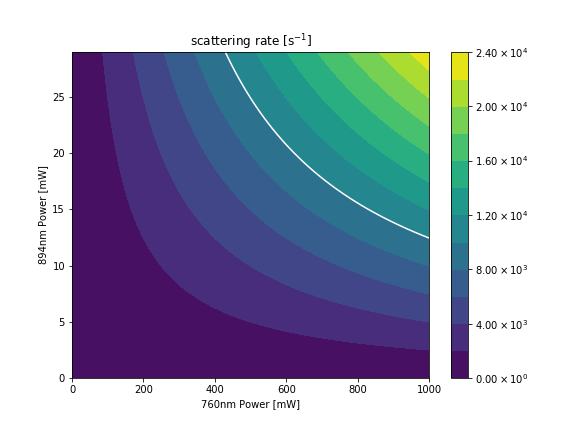
\includegraphics[keepaspectratio,  scale=0.6,  angle=0]
                          {figures/chapter3/2dcolor/5THz-16GHz-04GHz_new.png}
                          \caption{$f_\mathrm{rep} = 1.6\ \mathrm{GHz}$で$6P_{\frac{1}{2}}$と最近接の一光子コムの歯の離調が$400$ MHzのときの、二光子励起効率のパワー依存性。図中の白い実線が$10000\ \mathrm{s^{-1}}$の励起効率を示す。}

                          \label{5THz-16GHz-04GHz_new}
      \end{minipage}\\
        \begin{minipage}{1\hsize}
          \centering
            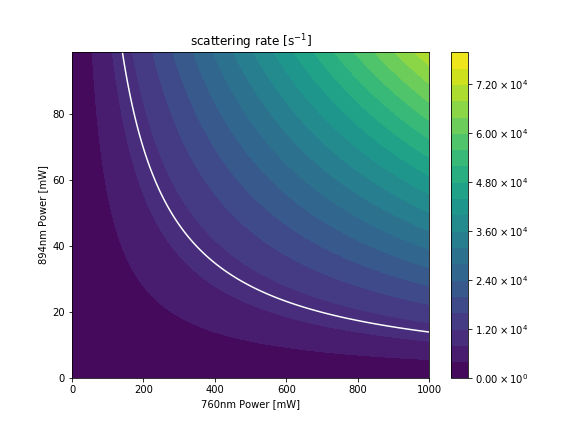
\includegraphics[keepaspectratio,  scale=0.6,  angle=0]
                            {figures/chapter3/2dcolor/5THz-16GHz-08GHz_new.png}
                            \caption{$f_\mathrm{rep} = 1.6\ \mathrm{GHz}$で$6P_{\frac{1}{2}}$と最近接の一光子コムの歯の離調が$800$ MHzのときの、二光子励起効率のパワー依存性。図中の白い実線が$10000\ \mathrm{s^{-1}}$の励起効率を示す。}
                            \label{5THz-16GHz-08GHz_new}
        \end{minipage}
    \end{tabular}
\end{figure}

\begin{comment}
\newpage
  実験系の以下のパラメータを用いて二色のコムでの励起効率の計算を行った。
\begin{itemize}
  \item 遷移 : 6sから8s
  \item 8S順位の線幅 : $2\pi \times 2.18$ MHz
  \item レーザービームの直径 : $0.5$ mm
  \item 760nm付近の波長を持つコムの強度 : $1$ W
  \item 894nm付近の波長を持つコムの強度 : $10$ mW
  \item コムの繰り返し周波数 : $1.6$ GHz
  \item 中間状態にもっとも近い二光子コムの歯の$6P_{\frac{3}{2}}$からの離調が$2 \mathrm{GHz}$
\end{itemize}
 この条件で一光子コムの周波数幅を変化させて励起効率を計算すると、図\ref{2color_excitation_rate}のようになった。切り出す周波数幅を大きくすると、中間状態からの離調が大きくなる分、励起効率が落ちることがわかる。ただし、切り出す周波数幅を小さくするとコムの強度も落ちるが、この効果は計算に取り入れられていない。

\begin{figure}[htbp]
 \begin{center}
  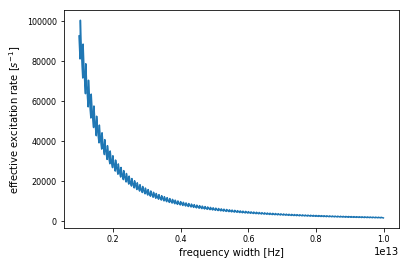
\includegraphics[width=100mm]{figures/chapter3/2color_excitation_rate_astro.png}
 \end{center}
 \caption{二光子励起効率の一光子コムの周波数幅に対する依存性}
 \label{2color_excitation_rate}
\end{figure}
\end{comment}

\bibliography{reference}

\end{document}
